% !TEX TS-program = pdflatex
% !TEX encoding = UTF-8 Unicode

% This file is a template using the "beamer" package to create slides for a talk or presentation
% - Talk at a conference/colloquium.
% - Talk length is about 20min.
% - Style is ornate.

% MODIFIED by Jonathan Kew, 2008-07-06
% The header comments and encoding in this file were modified for inclusion with TeXworks.
% The content is otherwise unchanged from the original distributed with the beamer package.

\documentclass{beamer}


% Copyright 2004 by Till Tantau <tantau@users.sourceforge.net>.
%
% In principle, this file can be redistributed and/or modified under
% the terms of the GNU Public License, version 2.
%
% However, this file is supposed to be a template to be modified
% for your own needs. For this reason, if you use this file as a
% template and not specifically distribute it as part of a another
% package/program, I grant the extra permission to freely copy and
% modify this file as you see fit and even to delete this copyright
% notice. 


\mode<presentation>
{
  \usetheme{Warsaw}
  % or ...

  \setbeamercovered{transparent}
  % or whatever (possibly just delete it)
}

%\usepackage{hyperref}
%\usepackage{url}

\usepackage{graphics}

\usepackage[english]{babel}
% or whatever

\usepackage[utf8]{inputenc}
% or whatever

\usepackage{times}
\usepackage[T1]{fontenc}
% Or whatever. Note that the encoding and the font should match. If T1
% does not look nice, try deleting the line with the fontenc.
\newcommand*{\newblock}{}
\usepackage[round]{natbib}
\bibliographystyle{apalike}

\title[GAM Revisited] % (optional, use only with long paper titles)
{Putting the Geographical Analysis Machine on the Internet Revisited}

%\subtitle{Include Only If Paper Has a Subtitle}

\author[Turton, Turner] % (optional, use only with lots of authors)
{\href{http://www.ccg.leeds.ac.uk/people/i.turton/}{Ian~Turton\inst{1}} \and \href{http://www.geog.leeds.ac.uk/people/a.turner/}{Andy Turner}\inst{2}}
% - Give the names in the same order as the appear in the paper.
% - Use the \inst{?} command only if the authors have different
%   affiliation.

\institute[ ] % (optional, but mostly needed)
{
  \inst{1}%
Independent Researcher\\
%  \href{mailto:ijturton@gmail.com}{ijturton@gmail.com}
  ijturton@gmail.com
  \and
  \inst{2}%
  \href{http://www.ccg.leeds.ac.uk/}{Centre for Computational Geography}\\
  \href{http://www.leeds.ac.uk/}{University of Leeds}\\
%  \href{mailto:A.G.D.Turner@leeds.ac.uk}{A.G.D.Turner@leeds.ac.uk}}
  A.G.D.Turner@leeds.ac.uk}
% - Use the \inst command only if there are several affiliations.
% - Keep it simple, no one is interested in your street address.

\date[ ] % (optional, should be abbreviation of conference name)
{\href{http://standard.cege.ucl.ac.uk/workshops/Geocomputation/}{GeoComputation 2011}}
% - Either use conference name or its abbreviation.
% - Not really informative to the audience, more for people (including
%   yourself) who are reading the slides online


% If you have a file called "university-logo-filename.xxx", where xxx
% is a graphic format that can be processed by latex or pdflatex,
% resp., then you can add a logo as follows:

% \pgfdeclareimage[height=0.5cm]{university-logo}{university-logo-filename}
% \logo{\pgfuseimage{university-logo}}



% Delete this, if you do not want the table of contents to pop up at
% the beginning of each subsection:
\AtBeginSubsection[]
{
  \begin{frame}<beamer>{Outline}
    \tableofcontents[currentsection,currentsubsection]
  \end{frame}
}


% If you wish to uncover everything in a step-wise fashion, uncomment
% the following command: 

%\beamerdefaultoverlayspecification{<+->}


\begin{document}


\begin{frame}
  \titlepage
\end{frame}


\begin{frame}{Outline}
  \tableofcontents
  % You might wish to add the option [pausesections]
\end{frame}


\section{Introduction}

\begin{frame}[t]
\frametitle{Introduction I}
\begin{itemize}
  \item Geographical Clustering
  \begin{itemize}
    \item Takes into account two variables 
    \item Essentially where one variables is unusually high, given the value of the other variable which is assumed to have a positively correlated distribution of values 
  \end{itemize}
\end{itemize}
\end{frame}

\begin{frame}[t]
\frametitle{Introduction II}
\begin{itemize}
  \item Space-time attribute pattern analysers
  \begin{itemize}
    \item Pioneered and developed by \href{http://www.ccg.leeds.ac.uk/people/s.openshaw/}{Stan Openshaw} and colleagues
    \item There are perhaps too many different kinds to summarise in a 20 minute presentation!
  \end{itemize}
\end{itemize}
\end{frame}

\begin{frame}[t]
\frametitle{Introduction III}
\begin{itemize}
  \item GAM
  \begin{itemize}
    \item The first Geographical Analysis Machine (GAM) was an early attempt to automate the search for geographical clusters (developed in the late 1980s)
    \item Generalised data of incidence and exposure (population at risk) across a range of scales (for overlapping circular sub-regions of different sizes) at a high resolution across the entire region
    \item Applied to find clusters of cancer
    \item Produced exciting and interesting results
  \end{itemize}
\end{itemize}
\end{frame}

\begin{frame}[t]
\frametitle{Introduction IV}
\begin{columns}
  \column{.5\textwidth}
    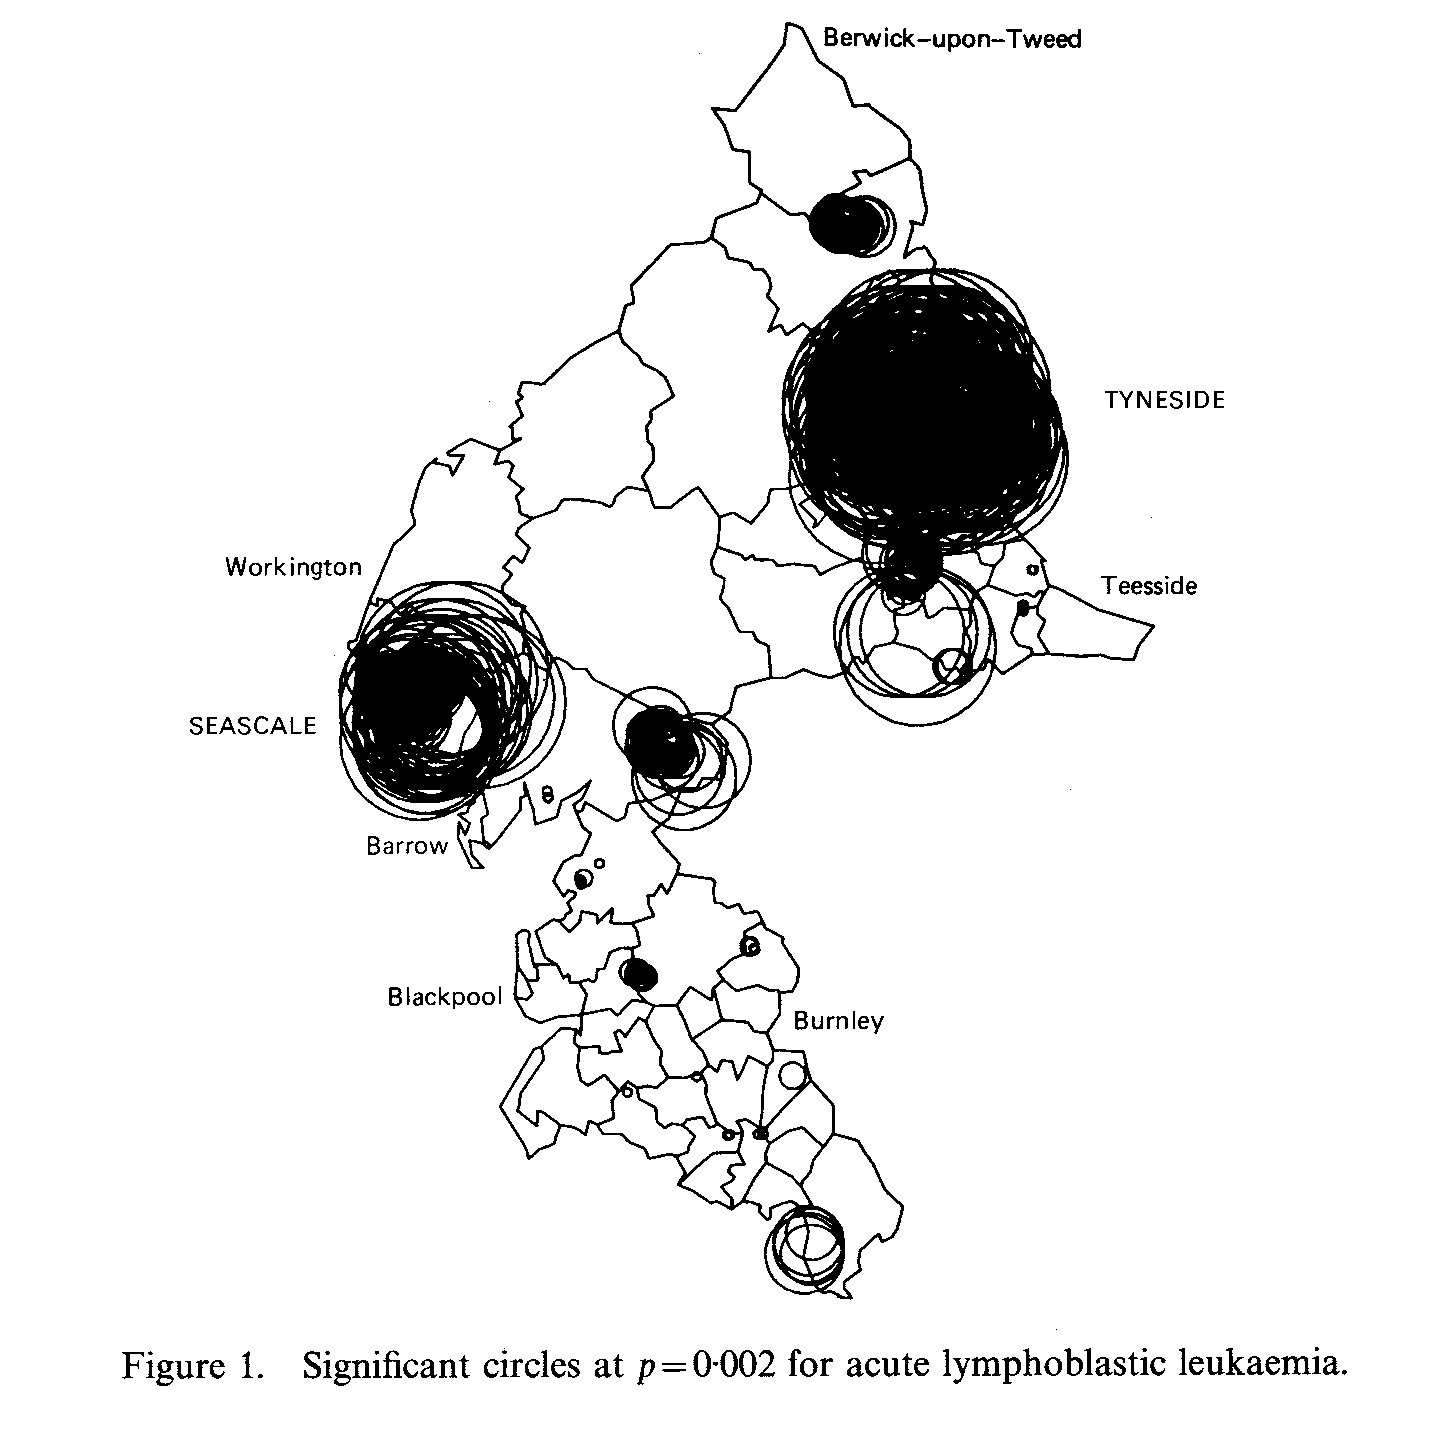
\includegraphics[height=6.0cm]{first_gam.png}
  \column{.5\textwidth}
%    \begin{itemize}
%      \item From \citet{citeulike:5207314}
%      \item First versions of GAM plotted circles with excess rates
%    \end{itemize}
    From \citet{citeulike:5207314}
\end{columns}
\end{frame}

\begin{frame}[t]
\frametitle{Introduction V}
\begin{itemize}
  \item GAM/K
  \begin{itemize}
    \item Generalised GAM results into a raster making it easier to identify the location and intensity of geographical clustering
    \item Optionally allowed for negative geographical clustering to be mapped whereby the other tail of the distribution of rates is plotted
    \begin{itemize}
      \item Where the values of one variable are unusually low, given the value of the other variable which is assumed to have a positively correlated distribution of values
    \end{itemize}
    \item An interface to GAM/K Fortran programs was made available on the World Wide Web (in the late 1990s)
    \begin{itemize}
      \item An attempt to bring tools to wider audience
%      \item Relied on
%      \begin{itemize}
%        \item Trust for uploading data
%        \item \href{http://www.ccg.leeds.ac.uk/}{CCG} computational infrastructure
%      \end{itemize}
      \item Relied on trust for uploading data
      \item Relied on \href{http://www.ccg.leeds.ac.uk/}{CCG} computational infrastructure
    \end{itemize}
  \end{itemize}
\end{itemize}
\end{frame}

\begin{frame}[t]
\frametitle{Introduction VI}
\begin{itemize}
  \item Cluster
  \begin{itemize}
    \item GAM/K re-implemented in Java
    \item Packaged with other clustering methods implemented in Java that shared the same code base
    \item Part of the SPIN System
    \begin{itemize}
      \item A spatial data mining system for data of public interest
    \end{itemize}
    \item Designed to be standalone
    \item Source code and executables made available on the web from 2003
  \end{itemize}
\end{itemize}
\end{frame}

\begin{frame}[t]
\frametitle{Introduction VII}
\begin{itemize}
  \item Further funding was not forthcoming and development came to a halt in 2003
  \item Cluster remained of interest and there were a considerable number of users that would give feedback and ask questions
  \item The Cluster code was getting old and in December 2010, on a whim Ian and I decided to refactor it and try to encourage the open development of a new generation of Geographical Information Systems based space-time attribute pattern analysers...
\end{itemize}
\end{frame}


\section{Motivation}

\begin{frame}[t]
\frametitle{Motivation I}
\begin{itemize}
  \item Earlier this year the Committee on Medical Aspects of Radiation in the Environment (\href{http://www.comare.org.uk/}{COMARE}) released it's fourteenth report \href{http://www.comare.org.uk/press_releases/documents/COMARE14report.pdf}{\textit{Further consideration of the incidence of childhood leukaemia around nuclear power plants in Great Britain}} which reported that there was no evidence of childhood cancer clusters around British nuclear power plants.
  \item Does anyone believe this?
\end{itemize}
\end{frame}

\begin{frame}[t]
\frametitle{Motivation II}
\begin{itemize}
  \item Epidemiologists need powerful tools to help them find clusters of diseases in the large databases that they collect.
  \item Current tools are hard to use, esoteric setup and formats to be mastered
  \begin{itemize}
    \item \citet{citeulike:6854836} state that "...training and software availability were cited as the primary barriers to the uptake of space-time disease surveillance..." and provide a general assessment that for the programs they tested - handling the data formatting was difficult and the interpretation of outputs was challenging.
  \end{itemize}
  \item So can we create a simple turn key tool set that allows them to run sophisticated analysis at the press of a button?
\end{itemize}
\end{frame}


\section{Implementation}

\begin{frame}[t]
\frametitle{Web Map Server (WMS)}
\begin{itemize}
  \item An Open Geospatial Consortium (\href{http://www.opengeospatial.org/}{OGC}) standard for the serving and consuming of geographical map images and raster data
  \begin{itemize}
    \item \href{http://www.opengeospatial.org/standards/wms}{http://www.opengeospatial.org/standards/wms}
  \end{itemize}
  \item Ideal for end users with little or no GIS experience
  \item Can be readily layered with other geographical data served in standard ways
  \item \textbf{Refactoring is to optionally use WMS to provide a feed and access to analysis results in a controlled and standard way}
\end{itemize}
\end{frame}

\begin{frame}[t]
\frametitle{Web Feature Server (WFS)}
\begin{itemize}
  \item An OGC standard for the serving and consuming of geographical feature data 
  \begin{itemize}
    \item \href{http://www.opengeospatial.org/standards/wfs}{http://www.opengeospatial.org/standards/wfs}
  \end{itemize}
  \item Useful for sharing vector data from a central repository to many users
  \item \textbf{Refactoring is to optionally be able to use WFS for feeding in the inputs for analysis}
\end{itemize}
\end{frame}

\begin{frame}[t]
\frametitle{Web Processing Standard (WPS)}
\begin{itemize}
  %\item An OGC standard \citep{OGC2007} that provides a defined protocol for executing remote processes on geographic data.
  \item An OGC standard that provides a defined protocol for executing remote processes on geographic data
  \begin{itemize}
    \item \href{http://www.opengeospatial.org/standards/wps}{http://www.opengeospatial.org/standards/wps}
  \end{itemize}
  \item Can take inputs from WFS servers or local files
  \item Advanced users can define a sub WPS process to produce the population at risk using a model.
  \item Returns results as downloadable files or via a WMS
\end{itemize}
\end{frame}

\begin{frame}[t]
\frametitle{GeoTools}
\begin{itemize}
  \item GeoTools is an open source Java library for geospatial operations \citep{Hall2008}
  \item GeoTools provides an abstracted datastore model, simple features and a variety of OGC standards (Filtering, Styling etc).
  \item Code and documentation are available at \url{http://geotools.org}
\end{itemize}
\end{frame}

\begin{frame}[t]
\frametitle{GeoServer}
\begin{itemize}
  \item High quality WMS/WFS/WCS/WPS
  \item used to serve up maps by many European NMA (GB,FR,NL...)
  \item Based on the GeoTools code base so integration is easy
  \item Download it and try for your self from \url{http://geoserver.org}
\end{itemize}
\end{frame}

\begin{frame}[t]
\frametitle{Clustering Code}
\begin{itemize}
  \item First developed under ESRC funding in FORTRAN
  \item Rewritten in Java under EU Spin! grant
  \item Now completely rewritten to use GeoTools and WPS processing tools
  \item Go to \url{http://code.google.com/p/spatial-cluster-detection/} to try out the code and join us in development... 
\end{itemize}
\end{frame}


\section{Results}

\begin{frame}[t]
\frametitle{England and Wales Crime Statistics}
\begin{itemize}
  \item In January 2011 the UK Government released geocoded crime statistics for England and Wales (\url{http://police.gov.uk}). 
  \item Many Heat maps were generated 
  \item Top 10 (or 100) lists were generated
  \item Almost none of these told us anything about crime
\end{itemize}
\end{frame}

\begin{frame}[t]
\frametitle{A Crime Heat map}
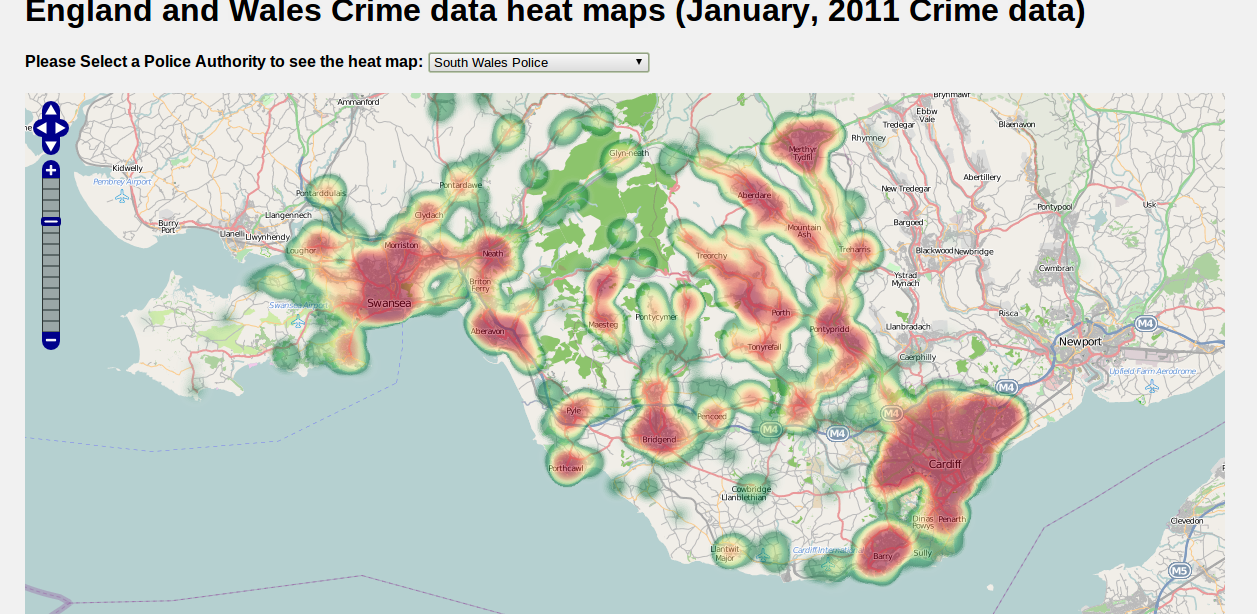
\includegraphics[height=6.0cm]{HeatMap.png}
From \href{http://www.gis-tech.co.uk/CrimeHeatMap/main.html}{http://www.gis-tech.co.uk/CrimeHeatMap/main.html}
\end{frame}

\begin{frame}[t]
\frametitle{GAM/K Analysis of Burglary Data}
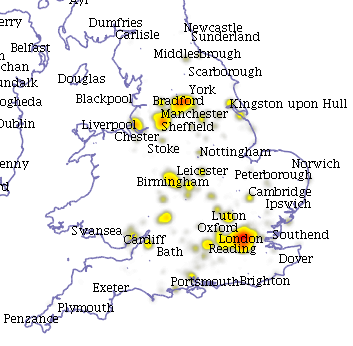
\includegraphics[height=6.0cm]{gam_burglary.png}
\end{frame}

\begin{frame}[t]
\frametitle{GAM/K Analysis of Robbery Data}
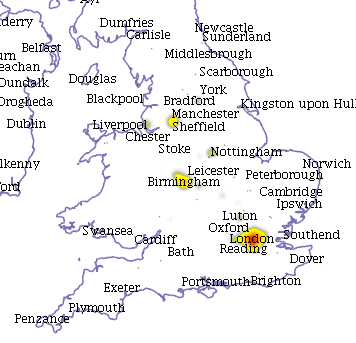
\includegraphics[height=6.0cm]{gam_robbery.png}
\end{frame}

\begin{frame}[t]
\frametitle{GAM/K Analysis of ASBO Data}
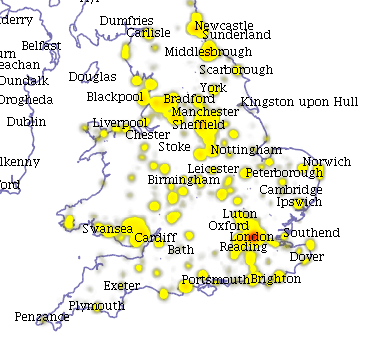
\includegraphics[height=6.0cm]{gam_asbo.png}
\end{frame}


\section{Conclusion}

\begin{frame}[t]
\frametitle{Conclusions}
\begin{itemize}
  \item It works
  \item It needs more work 
  \item Are you interested?
  \item Would you like to help?
  \item Please give us feedback and get involved
  \item Go to \href{http://code.google.com/p/spatial-cluster-detection/}{http://code.google.com/p/spatial-cluster-detection/}
\end{itemize}
\end{frame}

\begin{frame}[allowframebreaks]
\frametitle<presentation>{For Further Reading}    
\bibliography{clustering,ogc}
\end{frame}

\begin{frame}[t]
\frametitle{Feedback}
\begin{itemize}
  \item Thank you!
  \item Enjoy the rest of \href{http://standard.cege.ucl.ac.uk/workshops/Geocomputation/}{GeoComputation 2011}
  \item Andy's notes are on-line via \href{http://bit.ly/nIKMyB}{http://bit.ly/nIKMyB/}
\end{itemize}
\end{frame}


\end{document}
